\section{Analysis}
%
\begin{figure}%
  \def\frac{0.5}
  \begin{minipage}[b]{0.5\linewidth}
    \centering
    % Ours with and without step loss
    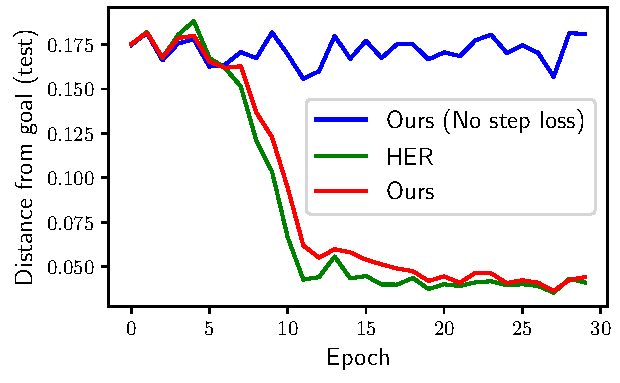
\includegraphics[width=\frac\columnwidth]{media/res/ablate-ddpg-with-without-step-loss/FetchPush-6efc1de-ddpgepoch-test/ag_g_dist.pdf}%
    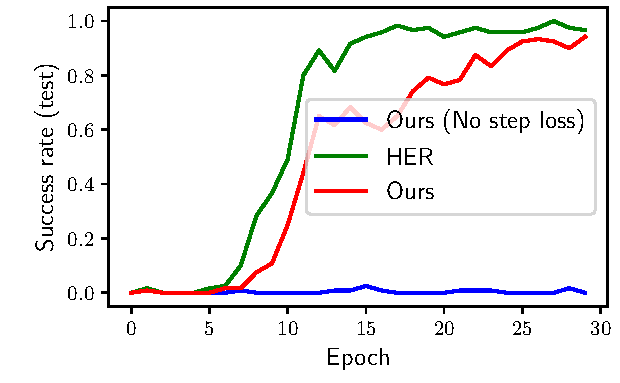
\includegraphics[width=\frac\columnwidth]{media/res/ablate-ddpg-with-without-step-loss/FetchPush-6efc1de-ddpgepoch-test/success_rate.pdf}\\
    \subcaption{Do we really need the step-loss?}
    \label{fig:with-and-without-step-loss-a}
  \end{minipage}
  \begin{minipage}[b]{0.5\linewidth}
    \centering
    % Ours with and without goal rewards
    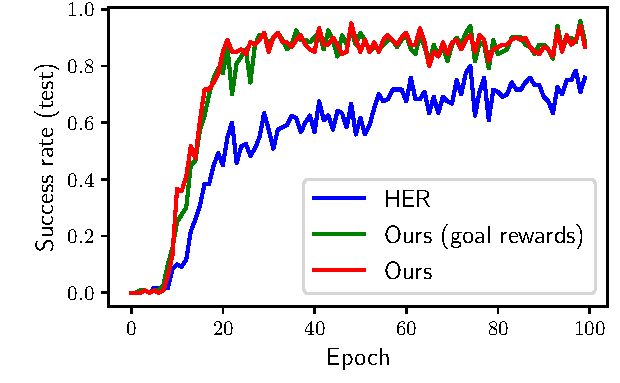
\includegraphics[width=\frac\columnwidth]{media/res/ablate-ours-with-goal-reward/FetchPickAndPlace-dqstepoch-test/success_rate.pdf}%
    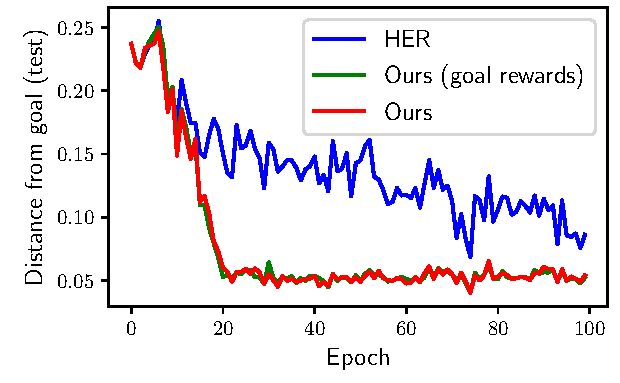
\includegraphics[width=\frac\columnwidth]{media/res/ablate-ours-with-goal-reward/FetchPickAndPlace-dqstepoch-test/ag_g_dist.pdf}\\
    \subcaption{Effect of goal-rewards}
    \label{fig:with-and-without-step-loss-b}
  \end{minipage}
  \caption{
      (a) Effects of removing the step-loss from our methods. Results
      show that it is a critical component to learning in the absence
      of goal-rewards.  
      (b) Adding goal-rewards to our algorithm that does have an effect
      further displaying how they are avoidable. 
    }
  \label{fig:with-and-without-step-loss}%
\end{figure}%
% 

%
\begin{figure}%
  \def\frac{0.5}
\begin{minipage}[b]{\frac\linewidth}\centering
  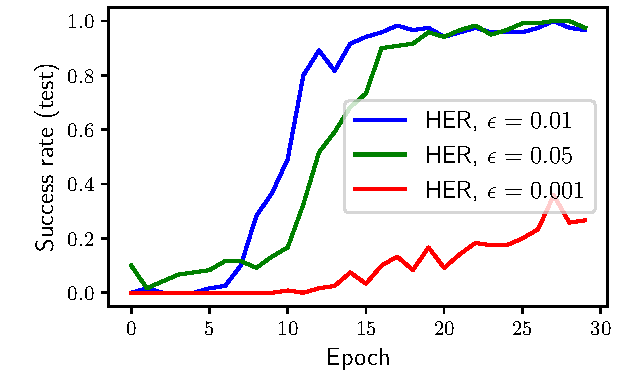
\includegraphics[width=\frac\columnwidth]{media/res/ablate-ddpg-dqst-low_tresh_chosen-low_thresh_alt-ddpg/0.05-be0910cepoch-test/success_rate.pdf}%
  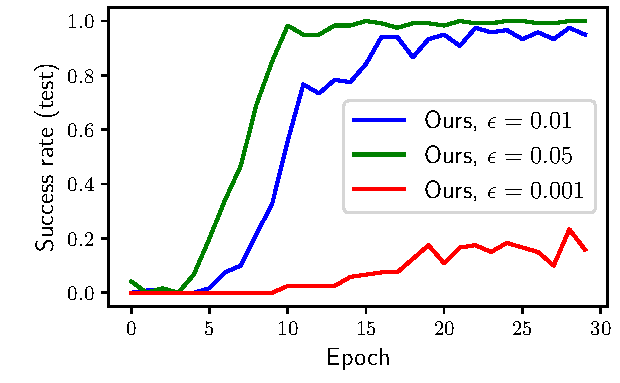
\includegraphics[width=\frac\columnwidth]{media/res/ablate-ddpg-dqst-low_tresh_chosen-low_thresh_alt-dqst/0.001-FetchPushPR-be467dfepoch-test/success_rate.pdf}%
  \subcaption{Sucesss rate}\label{fig:success-rate}
  \end{minipage}\begin{minipage}[b]{\frac\linewidth}\centering
  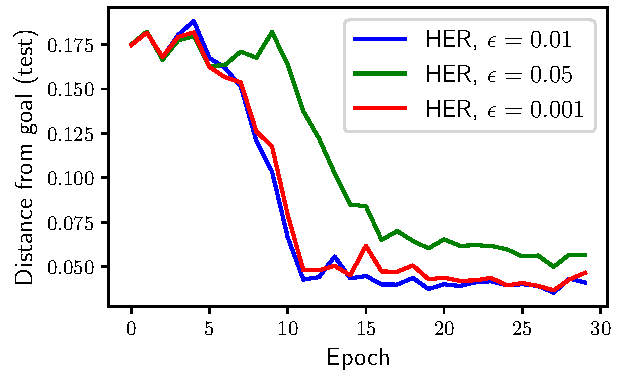
\includegraphics[width=\frac\columnwidth]{media/res/ablate-ddpg-dqst-low_tresh_chosen-low_thresh_alt-ddpg/0.05-be0910cepoch-test/ag_g_dist.pdf}%
  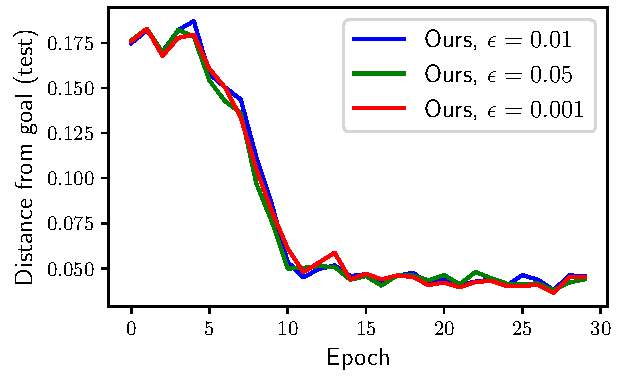
\includegraphics[width=\frac\columnwidth]{media/res/ablate-ddpg-dqst-low_tresh_chosen-low_thresh_alt-dqst/0.001-FetchPushPR-be467dfepoch-test/ag_g_dist.pdf}%
  \subcaption{Distance from goal}\label{fig:distance}
\end{minipage}
  \caption{We measure the sensitive of HER and our method to the
    dsitance-threshold ($\epsilon$) with respect to the success-rate
    and distance-from-goal metrics. Both algorithms success-rate is
    sensitive the threshold while only HER's distance-from-goal is
    affected by it. 
}%
  \label{fig:with-different-distance-thresholds}%
\end{figure}%
% 

To gain a deeper understanding of the method we perform three additional
experiments on different tasks. We ask the following questions:
(a) How important is the step loss?
(b) What happens when the goal-reward is also available to our method?
(c) How sensitive is HER and our method to the distance-threshold?
\paragraph{How important is the step loss?}
%
We choose the Fetch-Push task for this experiment.
We run our algorithm with no goal reward and without the step loss on
this task. Results show that our algorithm fails to reach the goal when the
step-loss is removed (Fig.~\ref{fig:with-and-without-step-loss-a})
showing its necessity.

\paragraph{What happens when the goal-reward is also available to our method?}
We run this experiment on the Fetch PickAndPlace task. We find that
goal-rewards do not affect the performance of our algorithm further
solidifying the avoidability of goal-reward
(Fig~\ref{fig:with-and-without-step-loss-b}).

\paragraph{How sensitive is HER and our method to the distance-threshold?}
In the absence of goal-rewards, our algorithm is not to able capture distance
threshold information that decides whether the agent has reached the goal or
not. This information is available to HER. To understand the
sensitivity of our algorithm and HER on this parameter, we vary it over
0.05 (the original HER value), 0.01 and 0.001 meters
(Fig.~\ref{fig:with-different-distance-thresholds}). Results show that
for the success-rate metric, which is itself a function of this
parameter, both algorithms are affected equally
(Fig.~\ref{fig:success-rate}). 
For the distance-from-goal,
only HER is affected (Fig.~\ref{fig:distance}). This fits our expectations as set up in 
section~\ref{sec:hyperparams}.




